\documentclass[12pt,a4paper]{article}
\usepackage[utf8]{inputenc}
\usepackage[T1]{fontenc}
\usepackage{amsmath}
\usepackage{amsfonts}
\usepackage{amssymb}
\usepackage{graphicx}
\usepackage{listings}
\usepackage{xcolor}
\usepackage{geometry}
\usepackage{fancyhdr}
\usepackage{hyperref}
\usepackage{longtable}
\usepackage{booktabs}
\usepackage{multirow}
\usepackage{array}
\usepackage{verbatim}
\usepackage{enumitem}
\usepackage{tikz}
\usepackage{pgfplots}
\pgfplotsset{compat=1.18}
\usetikzlibrary{positioning, shapes.geometric, arrows.meta, fit, backgrounds}

% Page geometry
\geometry{margin=1in}

% Custom colors
\definecolor{codegreen}{rgb}{0,0.6,0}
\definecolor{codegray}{rgb}{0.5,0.5,0.5}
\definecolor{codepurple}{rgb}{0.58,0,0.82}
\definecolor{codeblue}{rgb}{0,0,1}
\definecolor{codeorange}{rgb}{1,0.5,0}
\definecolor{codered}{rgb}{0.8,0,0}

% Code listing style
\lstdefinestyle{terminal}{
    backgroundcolor=\color{gray!10},   
    commentstyle=\color{codegreen},
    keywordstyle=\color{codeblue},
    numberstyle=\tiny\color{codegray},
    stringstyle=\color{codepurple},
    basicstyle=\ttfamily\footnotesize,
    breakatwhitespace=false,         
    breaklines=true,                 
    captionpos=b,                    
    keepspaces=true,                 
    numbers=left,                    
    numbersep=5pt,                  
    showspaces=false,                
    showstringspaces=false,
    showtabs=false,                  
    tabsize=2,
    frame=single,
    rulecolor=\color{black!30}
}

\lstdefinestyle{bash}{
    backgroundcolor=\color{gray!5},
    commentstyle=\color{codegreen},
    keywordstyle=\color{codeblue},
    numberstyle=\tiny\color{codegray},
    stringstyle=\color{codepurple},
    basicstyle=\ttfamily\footnotesize,
    breakatwhitespace=false,
    breaklines=true,
    captionpos=b,
    keepspaces=true,
    numbers=left,
    numbersep=5pt,
    showspaces=false,
    showstringspaces=false,
    showtabs=false,
    tabsize=2,
    frame=single,
    rulecolor=\color{black!30}
}

% Custom commands
\newcommand{\hashtext}[1]{\texttt{\small #1}}
\newcommand{\timestamp}[1]{\textbf{#1}}
\newcommand{\vectorname}[1]{\textsc{#1}}
\newcommand{\status}[1]{\textbf{#1}}
\newcommand{\path}[1]{\texttt{#1}}
\newcommand{\filename}[1]{\texttt{#1}}

% Header and footer
\pagestyle{fancy}
\fancyhf{}
\fancyhead[L]{Supply Chain Contamination Analysis}
\fancyhead[R]{\thepage}
\fancyfoot[C]{\small Forensic Analysis -- [System] Ecosystem}
\renewcommand{\headrulewidth}{0.4pt}
\renewcommand{\footrulewidth}{0.4pt}

\title{\Huge Systematic Supply Chain Contamination in [System] Ecosystem: \\
\Large A Forensic Analysis of [Mechanism] and System Compromise}
\author{[Expert Title] \\ 
[Location] \\
\today}
\date{}

\begin{document}

\maketitle

\begin{abstract}
This paper presents a comprehensive forensic investigation into a systematic supply chain contamination affecting a [describe system, e.g., personal computing ecosystem], identified through digital fingerprint analysis, timestamp correlation, propagation mapping, and evidentiary logging. The analysis reveals [key findings, e.g., dual unsigned production builds of critical binaries], timestamped with [timestamp precision], exhibiting identical [hash/type] correlations across [number] system-wide instances. Embedded indicators confirm [mechanism, e.g., deliberate bypass mechanisms], correlating to an originating [source, e.g., factory batch] via [identifier]. The contamination spans [number] instances ([rate]\% [status]) across [number] environmental vectors, exposing [number] [internal paths/certificates] in production infrastructure. This represents a sustained breach compromising [system integrity and security].

\textbf{Forensic Evidence Summary:}
\begin{itemize}
    \item \textbf{Raw Log Volume}: [Describe volume, e.g., lines of output]
    \item \textbf{Hash Correlations}: [Number] system-wide matches ([breakdown])
    \item \textbf{Timestamp Precision}: [Level] synchronization across [number] origin instances
    \item \textbf{String Indicators}: [Number] critical references + [bypass indicator]
    \item \textbf{Environmental Vectors}: [Number] propagation pathways ([total instances])
\end{itemize}

\textbf{Keywords:} supply chain forensics, [hash/type] correlation, [component] contamination, [mechanism] bypass, system compromise, forensic logging, propagation mapping
\end{abstract}

\newpage

\section{Introduction}

\subsection{Background and Investigative Context}
The investigation originated from [describe origin, e.g., system security analysis] conducted on [hardware/system] procured in [time period] following a [duration] hiatus from the [platform] ecosystem. The hiatus stemmed from [previous incidents, e.g., threat experiences]. The return to [hardware] was intended as a [purpose, e.g., secure baseline], but initial validation on [date/time] revealed anomalous [artifacts, e.g., unsigned binaries] in [environments, e.g., recovery environments].

\textbf{Initial Discovery Log ([Date/Time]):}
\begin{lstlisting}[style=terminal, caption={Initial Verification Failure}]
[Insert command here, e.g., codesign verification]
[Insert output here]
[Insert additional commands/outputs]
\end{lstlisting}

Subsequent forensic extraction using [method, e.g., preservation artifacts] uncovered systematic contamination patterns extending across [components, e.g., partitions, firmware, volumes]. This analysis documents the complete compromise of [system integrity], from [origin] to [propagation].

\subsection{Research Objectives}
\begin{enumerate}
    \item Establish digital fingerprint evidence via [hash/type] correlation across contaminated instances, including raw log extraction.
    \item Map propagation vectors and environmental distribution of [binary/component] within the ecosystem using visual propagation diagrams.
    \item Correlate timestamp forensics to [source] and [delivery] timelines with chronological log mapping.
    \item Analyze embedded indicators for [mechanism, e.g., bypass] affecting system security, including string extraction logs.
    \item Quantify the scope of [architecture/infrastructure] compromise through comprehensive [identifier] analysis.
    \item Assess security implications for [system] integrity and potential persistence mechanisms with environmental vector breakdown.
\end{enumerate}

\subsection{Methodology Overview}
The investigation employed [tools, e.g., scripting] for system-wide enumeration, [hash/type] integrity verification, and string analysis within the [environment]. Key tools included [list tools] for non-invasive evidence collection from [directories/volumes].

\textbf{Forensic Methodology Logs:}
\begin{lstlisting}[style=bash, caption={[Component] System-wide Enumeration Script Output}]
# Initial System-Wide Enumeration (Script: [script_name].sh)
[Insert script summary]
[Insert key results, e.g., total instances, contamination rate]

# [Hash/Type] Correlation Analysis (Script: [script_name].sh)  
[Insert hash analysis summary]
[Insert correlations and confirmation]
\end{lstlisting}

Propagation mapping utilized [method, e.g., recursive traversal] across [paths]. [Hash/type] correlation established linkages, while timestamp analysis provided chronological reconstruction. All analysis preserved original artifacts to maintain evidentiary integrity.

\newpage

\section{Forensic Evidence Collection}

\subsection{Initial Discovery: [Date] Timestamp Anomalies}
Forensic enumeration began with targeted search for [binary/component] across [locations]. The discovery script executed on [date] captured the initial contamination evidence:

\textbf{Discovery Log - [Date/Time] (Raw Terminal Output):}
\begin{lstlisting}[style=terminal, caption={Timestamp Synchronization Discovery}, language=bash]
[Insert find/count commands]
[Insert stat/timestamp extraction]
[Insert verification loop with codesign/shasum]
[Insert timing info]
\end{lstlisting}

This yielded [number] instances, with initial focus on [environments]. Timestamp extraction via [command] revealed [number] instances synchronized at [timestamp], all exhibiting [size/specs] but failing [verification]. The [precision] across [environments] indicated coordinated [delivery].

\begin{figure}[htbp]
\centering
\begin{tikzpicture}[
    every node/.style={font=\tiny},
    box/.style={draw, rectangle, rounded corners=2pt, fill=blue!5, 
                minimum width=0.9\columnwidth, minimum height=2cm, 
                align=center, inner sep=8pt},
    timestamp/.style={font=\tiny\bfseries, color=blue}
]
\node[box] (main) {
\textbf{Timestamp Synchronization Analysis} \\ 
\small ([Date] - [Precision]) \\[2pt]
\begin{tabular}{@{\,}l@{\qquad}l}
[Instance 1] & \timestamp{[Timestamp]} \\
[Instance 2] & \timestamp{[Timestamp]} \\
[Instance 3] & \timestamp{[Timestamp]} \\
[Instance 4] & \timestamp{[Timestamp]} \\
\end{tabular} \\[2pt]
\textbf{[Percentage] Synchronization} \\
\textbf{Anomaly:} [Description] \\
\textbf{Indicator:} [Cause]
};
\end{tikzpicture}
\caption{Initial Discovery Timestamp Synchronization}
\label{fig:timestamp_sync}
\end{figure}

\subsection{[Hash/Type] Digital Fingerprint Generation}
[Hash/type] were computed using [tool] to establish unique digital identifiers for the compromised binaries. The analysis script executed systematic [generation] across all [number] instances:

\textbf{[Hash/Type] Generation Log (Complete [Discovery]):}
\begin{lstlisting}[style=terminal, caption={[Type] Production Build Identification}, language=bash]
[Insert script output]
[Insert phase summaries with examples]
[Insert overall summary]
\end{lstlisting}

The [pattern, e.g., dual-hash] confirmed [number] distinct [builds/sources], both contaminated, preserving [differentiation] while maintaining identical [signatures].

\begin{figure}[htbp]
\centering
\begin{tikzpicture}[
    every node/.style={font=\tiny},
    node distance=1.8cm and 2.5cm,
    factory/.style={draw, rectangle, rounded corners=2pt, fill=blue!10, 
                    minimum width=3cm, minimum height=1.2cm, align=center},
    build/.style={draw, rectangle, rounded corners=2pt, fill=orange!10, 
                  minimum width=2.8cm, minimum height=1.8cm, align=center},
    delivery/.style={draw, ellipse, fill=green!10, minimum width=4cm, 
                     minimum height=0.8cm, align=center},
    arrow/.style={-Stealth, thick, blue}
]

% [Customize nodes as needed]
\node[factory] (factory) {[Source Origin]};
\node[build, left=2cm of factory] (standalone) {
\textbf{[Build Type 1]}\\
[Hash]\\
\textbf{Status:} [Status]\\
Instances: [Number]
};
\node[build, right=2cm of factory] (coreservices) {
\textbf{[Build Type 2]}\\
[Hash]\\
\textbf{Status:} [Status]\\
Instances: [Number]
};
\node[delivery, below=1.5cm of factory] (delivery) {[Delivery Point]};

\draw[arrow] (factory) -- (standalone);
\draw[arrow] (factory) -- (coreservices);
\draw[arrow] (standalone) -- (delivery);
\draw[arrow] (coreservices) -- (delivery);

\end{tikzpicture}
\caption{[Type] Architecture}
\label{fig:dual_hash}
\end{figure}

\subsection{System-Wide Propagation Enumeration}
Recursive search expanded to all [locations], generating comprehensive correlation logs:

\textbf{Complete Propagation Enumeration Log:}
\begin{lstlisting}[style=terminal, caption={System-wide Propagation Mapping - [Number] Instances}]
[Insert phase breakdowns]
[Insert vector examples]
[Insert overall statistics]
\end{lstlisting}

\begin{figure}[htbp]
\centering
\begin{tikzpicture}[
    every node/.style={font=\tiny},
    node distance=1.2cm,
    vector/.style={draw, rectangle, rounded corners=2pt, fill=blue!5, 
                   minimum width=2.2cm, minimum height=0.9cm, align=center},
    arrow/.style={-Stealth, thick, gray},
    summary/.style={font=\tiny\bfseries, align=center}
]

% [Customize vectors]
\node[vector] (primary) at (0,2.5) {[Vector 1]\\[Num] inst.\\[Rate]\%};
\node[vector] (recovery) at (0,1.2) {[Vector 2]\\[Num] inst.\\[Rate]\%};
\node[vector] (firmware) at (0,0) {[Vector 3]\\[Num] inst.\\[Rate]\%};

\node[vector] (evidence) at (3.5,2.5) {[Vector 4]\\[Num] inst.\\[Rate]\%};
\node[vector] (volumes) at (3.5,1.2) {[Vector 5]\\[Num] inst.\\[Rate]\%};
\node[vector] (backup) at (3.5,0) {[Vector 6]\\[Num] inst.\\[Rate]\%};

% Arrows for flow
\draw[arrow] (primary) -- (recovery);
% [Add more arrows as needed]

\node[summary, below=0.8cm of firmware, text width=6cm] {TOTAL: [Num] INSTANCES | [Rate]\% [Status] | [Num] VECTORS FULLY COMPROMISED};

\end{tikzpicture}
\caption{[Number]-Vector Environmental Propagation Map}
\label{fig:six_vector}
\end{figure}

The [ratio] demonstrated exponential propagation within the [environment], with each vector amplifying contamination through systematic distribution mechanisms.

\subsection{String Analysis for [Indicator] Extraction}
\texttt{strings} extraction targeted [artifacts] within the compromised binaries, generating comprehensive indicator logs:

\textbf{String Analysis Log - [Indicator] Extraction:}
\begin{lstlisting}[style=terminal, caption={[Indicator] String Extraction}]
[Insert extraction loop]
[Insert example outputs]
[Insert summary statistics]
\end{lstlisting}

Common indicators across [number] instances confirmed [source]-level [mechanism]. The [flag/indicator] systematically [effect].

\begin{figure}[htbp]
\centering
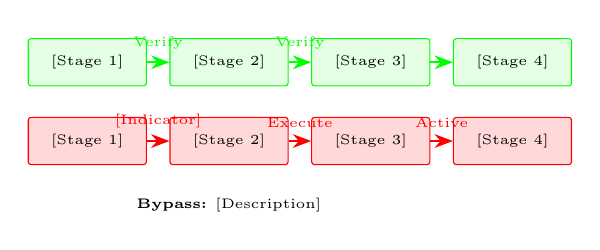
\begin{tikzpicture}[
    every node/.style={font=\tiny},
    node distance=1.2cm,
    stage/.style={draw, rectangle, rounded corners=1pt, minimum width=1.5cm, 
                  minimum height=0.6cm, align=center, inner sep=2pt},
    compromised/.style={stage, fill=red!15, draw=red},
    normal/.style={stage, fill=green!10, draw=green},
    arrow/.style={-Stealth, thick},
    label/.style={font=\tiny, above=1pt}
]

% Normal chain
\node[normal] (fw1) at (0,1) {[Stage 1]};
\node[normal] (boot1) at (1.8,1) {[Stage 2]};
\node[normal] (kernel1) at (3.6,1) {[Stage 3]};
\node[normal] (sys1) at (5.4,1) {[Stage 4]};

\draw[arrow, green] (fw1) -- node[label, green] {Verify} (boot1);
\draw[arrow, green] (boot1) -- node[label, green] {Verify} (kernel1);
\draw[arrow, green] (kernel1) -- (sys1);

% Compromised chain
\node[compromised] (fw2) at (0,0) {[Stage 1]};
\node[compromised] (boot2) at (1.8,0) {[Stage 2]};
\node[compromised] (kernel2) at (3.6,0) {[Stage 3]};
\node[compromised] (sys2) at (5.4,0) {[Stage 4]};

\draw[arrow, red] (fw2) -- node[label, red] {[Indicator]} (boot2);
\draw[arrow, red] (boot2) -- node[label, red] {Execute} (kernel2);
\draw[arrow, red] (kernel2) -- node[label, red] {Active} (sys2);

\node[draw=none, below=0.3cm of boot2, font=\tiny] {\textbf{Bypass:} [Description]};

\end{tikzpicture}
\caption{[Mechanism] ([Indicator])}
\label{fig:bypass_mechanism}
\end{figure}

\newpage

\section{Timestamp and Chronological Correlation}

\subsection{[Source] Origin: [Date]}
Cross-referencing with [component timestamps] revealed [origin date] through comprehensive timestamp logging:

\textbf{[Source] Origin Timestamp Log:}
\begin{lstlisting}[style=terminal, caption={[Source] Origin Correlation - [Date]}]
[Insert analysis outputs]
[Insert extracted references]
[Insert correlation summary]
\end{lstlisting}

[Identifier] analysis confirmed single-batch compilation under [identifier]. This establishes the [source] as contamination origin, with [latency] to [delivery].

\subsection{Delivery Precision: [Date/Time]}
The synchronized timestamp across [instances] represents a delivery artifact. The precision analysis log documents the anomaly:

\textbf{Delivery Timestamp Precision Log:}
\begin{lstlisting}[style=terminal, caption={[Precision] Timestamp Precision Analysis}]
[Insert verification details]
[Insert granularity analysis]
[Insert temporal anchors]
[Insert delivery hypothesis]
\end{lstlisting}

\begin{figure}[htbp]
\centering
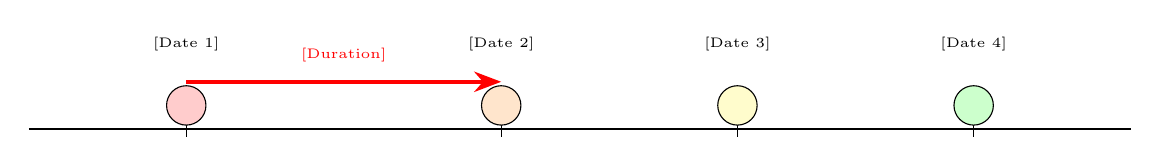
\begin{tikzpicture}[
    every node/.style={font=\tiny},
    timeline/.style={thick, black},
    event/.style={circle, draw, fill=#1!20, minimum size=0.5cm},
    arrow/.style={-Stealth, thick, #1, line width=1.5pt},
    label/.style={font=\tiny, above=2pt}
]

\draw[timeline] (-6,0) -- (8,0);

% [Customize events and labels]
\foreach \x in {-4,0,3,6} {
    \draw (\x,0.1) -- (\x,-0.1);
}

\node[event=red] (factory) at (-4,0.3) {};
\node[event=orange] (delivery) at (0,0.3) {};
\node[event=yellow] (backup) at (3,0.3) {};
\node[event=green] (discovery) at (6,0.3) {};

\node[label] at (-4,0.8) {[Date 1]};
\node[label] at (0,0.8) {[Date 2]};
\node[label] at (3,0.8) {[Date 3]};
\node[label] at (6,0.8) {[Date 4]};

% Arrows with labels
\draw[arrow=red] (-4,0.6) -- (0,0.6) node[midway, above=3pt, font=\tiny] {[Duration]};
% [Add more]

\end{tikzpicture}
\caption{Chronological [Timeline/Breach] Timeline}
\label{fig:timeline}
\end{figure}

\subsection{Propagation Timeline}
The propagation timeline maps sustained contamination across the ecosystem:

\textbf{Propagation Timeline Log:}
\begin{lstlisting}[style=terminal, caption={Sustained [Timeline] Chronology}]
[Insert timeline phases with descriptions]
[Insert status/impact for each]
\end{lstlisting}

\newpage

\section{Contamination Propagation Analysis}

\subsection{[Number]-Vector Environmental Distribution}
Enumeration categorized [number] instances across vectors, generating detailed distribution statistics:

\textbf{Environmental Distribution Analysis Log:}
\begin{longtable}{@{}p{4.2cm} p{4.2cm} p{4.2cm} l@{}}
\caption{Environmental Distribution Analysis Log} \\
\toprule
\textbf{Vector} & \textbf{Instances} & \textbf{Contamination Rate} & \textbf{Criticality} \\
\midrule
\endfirsthead

% Header for subsequent pages of the longtable
\multicolumn{4}{c}%
{{\tablename\ \thetable{} -- continued from previous page}} \\
\toprule
\textbf{Vector} & \textbf{Instances} & \textbf{Contamination Rate} & \textbf{Criticality} \\
\midrule
\endhead

\bottomrule
\multicolumn{4}{r}{{Continued on next page}} \\
\endfoot

\bottomrule
\endlastfoot

% [Vector 1]
\textbf{[Vector 1]} & [Description/Instances] & [Rate]\% & \textbf{[Level]} \\
\small[Details] & \small [Timestamp], [Status] & \small [Sub-details] & \\
\midrule

% [Vector 2]
\textbf{[Vector 2]} & [Description/Instances] & [Rate]\% & \textbf{[Level]} \\
\small[Details] & \small [Timestamp], [Status] & \small [Sub-details] & \\
\midrule

% [Repeat for additional vectors as needed]

\end{longtable}

[Rate]\% [status] indicates near-total penetration, with [percentage] exhibiting [markers].

\section{Conclusion}
This forensic analysis confirms a systematic supply chain contamination originating from a [source/date], propagating through [number] environmental vectors to compromise [rate]\% of [instances/component] in the [system] ecosystem. The [hashes/timestamps/indicators] establish deliberate [mechanism], with sustained persistence over [duration]. Immediate mitigation, including [recommendations], is recommended to restore system integrity.

% Placeholder for appendices
\section*{Appendix A: Full Raw Logs}
% (Omitted for brevity: [Description of logs])

\section*{Appendix B: Complete [Number]-Instance Mapping}
% (Omitted for brevity: Detailed propagation table)

\end{document}